\chapter{Seeing Unseeability to See the Unseeable}

\section{Introduction}
\label{sec:introduction}

\begin{quote}
  [T]here are known knowns; there are things we know we know.
  %
  We also know there are known unknowns; that is to say we know there are some
  things we do not know.
  %
  But there are also unknown unknowns --- the ones we don't know we don't know.
  \par\vspace*{-3ex}
  \begin{flushright}
    Donald Rumsfeld (12 February 2002)
  \end{flushright}
  \par\vspace*{-4ex}
\end{quote}

\noindent People exhibit the uncanny ability to see the unseeable.
%
The colloquial exhortation \emph{You have eyes in the back of your
  head!}\ expresses the assessment that someone is making correct judgments as
if they could see what is behind them, but obviously cannot.
%
People regularly determine the properties of occluded portions of objects from
observations of visible portions of those objects using general world knowledge
about the consistency of object properties.
%
Psychologists have demonstrated that the world knowledge that can influence
perception can be high level, abstract, and symbolic, and not just related to
low-level image properties such as object class, shape, color, motion, and
texture.
%
For example, \singleemcite{FreydPC88} showed that physical forces, such as
gravity, and whether such forces are in equilibrium, due to support and
attachment relations, influences visual perception of object location in adults.
%
\singleemcite{Baillargeon86,Baillargeon87} showed that knowledge of
substantiality, the fact that solid objects cannot interpenetrate, influences
visual object perception in young infants.
% Phil Kellman, Kestenbaum, Frank Keil, Larry Macomber, or ...someone in UMich
\singleemcite{Streri1988} showed that knowledge about object rigidity
influences both visual and haptic perception of those objects in young infants.
%
Moreover, such influence is cross modal: observable haptic perception
influences visual perception of unobservable properties and observable visual
perception influences haptic perception of unobservable properties.
% Karen Wynn UArizona
\singleemcite{Wynn1998} showed that material properties of objects, such as
whether they are countable or mass substances, along with abstract properties,
such as the number of countable objects and the quantity of mass substances, and
how they are transferred between containers, influences visual perception in
young infants.
%
Similar results exist for many physical properties such as relative mass,
momentum, etc.
%
These results demonstrate that people can easily integrate information from
multiple sources together with world knowledge to see the unseeable.

People so regularly invoke the ability to see the unseeable that we often don't
realize that we do so.
%
If you observe a person entering the front door of a house and later see them
appear from behind the house without seeing them exit, you easily see the
unseeable and conclude that there must be an unseen door to the house.
%
But if one later opens a curtain covering a large living-room bay window in the
front of the house so that you see through the house and see the back door you
no longer need to invoke the ability to see the unseeable.
%
A more subtle question then arises: when must you invoke the ability to see the
unseeable?
%
In other words how can you see unseeability, the inability to see?
%
This question becomes particularly thorny since, as we will see, it can
involve a chicken-and-egg problem: seeing the unseen can require seeing the
unseeability of the unseen and seeing the unseeability of the unseen can
require seeing the unseen.

The ability to see unseeability and to see the unseeable can further
dramatically influence human behavior.
%
We regularly and unconsciously move our heads and use our hands to open
containers to render seeable what was previously unseeable.
%
To realize that we need to do so in the first place, we must first see the
unseeability of what we can't see.
%
Then we must determine how to best use our perceptual, motor, and reasoning
affordances to remedy the perceptual deficiency.

We present a general computational framework for seeing unseeability to see the
unseeable.
%
We formulate and evaluate a particular instantiation of this general framework
in the context of a restricted domain, namely \LincolnLogs, a children's
assembly toy where one constructs assemblies from a small inventory of logs.
%
Two relevant aspects of this domain facilitate its use for investigating our
general computational framework: (a)~\LincolnLog\ assemblies suffer from
massive occlusion and (b)~a simple but rich expression of world knowledge, in
the form of constraints on valid assemblies, can mitigate the effects of such
occlusion.
%
While \LincolnLogs\ are a children's toy, this domain is far from a toy when it
comes to computer vision.
%
The task of structure estimation, determining, from an image, the correct
combination of component logs used to construct an assembly and how they are
combined, is well beyond the state of the art.
%
Not only is the computer-vision problem for this domain immensely
difficult---occlusion, luminance variation, and a distinct paucity of features
all encumber the process---the computational problem itself affords a richness
and complexity that is not readily apparent.

We present methods for seeing the unseeable (in Section~\ref{sec:structure})
and seeing unseeability (in Section~\ref{sec:visibility}) based on precise
computation of the maximum-likelihood structure estimate.
%
Section~\ref{sec:confidence} presents a rational basis for determining
confidence in one's structure estimate despite unseeability based on precise
computation of the amount of evidence needed to override a uniform prior on the
unseeable.
%
Section~\ref{sec:integration} presents an active-vision decision-making
process for determining rational behavior in the presence of unseeability based
on precise computation of which of several available perception-enhancing
actions one should take to maximally improve the confidence in one's structure
estimate.
%
Such capability is bootstrapped by our framework's capacity to integrate
evidence from different views, both \emph{imagined} and \emph{actual}.
%
Section~\ref{sec:language} further highlights the elegance of our framework by
demonstrating the integration of evidence \emph{across} modalities; using
natural-language descriptions to aid in resolving ambiguities in structure
estimation.

\par\vspace{-1ex}
\section{Structure Estimation}
\label{sec:structure}

Speech recognizers use a human language model, on utterances in a generative
linguistic domain, to improve recognition accuracy over the raw recognition
rate of the phoneme detectors.
%
Analogously, \singleemcite{Siddharth2011} use a visual language
model, on compositional visual structures in a generative visual domain, to
improve recognition accuracy over the raw recognition rate of the part
detectors.
%
In this approach, a complex object is constructed out of a collection of parts
taken from a small part inventory.
%
A language model, in the form of a stochastic constraint-satisfaction problem
(CSP; \npcite{Lauriere1978}), characterizes the constrained way object parts can
combine to yield a whole object and significantly improves the recognition rate
of the whole structure over the infinitesimally small recognition rate that
would result from unconstrained application of the unreliable part detectors.
%
Unlike the speech-recognition domain, where (except for coarticulation) there
is acoustic evidence for all phonemes, in the visual domain there may be
components with no image evidence due to occlusion.
%
A novel aspect of applying a language model in the visual domain instead of the
linguistic domain is that it can additionally help in recovering occluded
information.

\begin{figure}
  \centering
  \begin{tabular}{@{}c@{\hspace{2pt}}c@{}}
    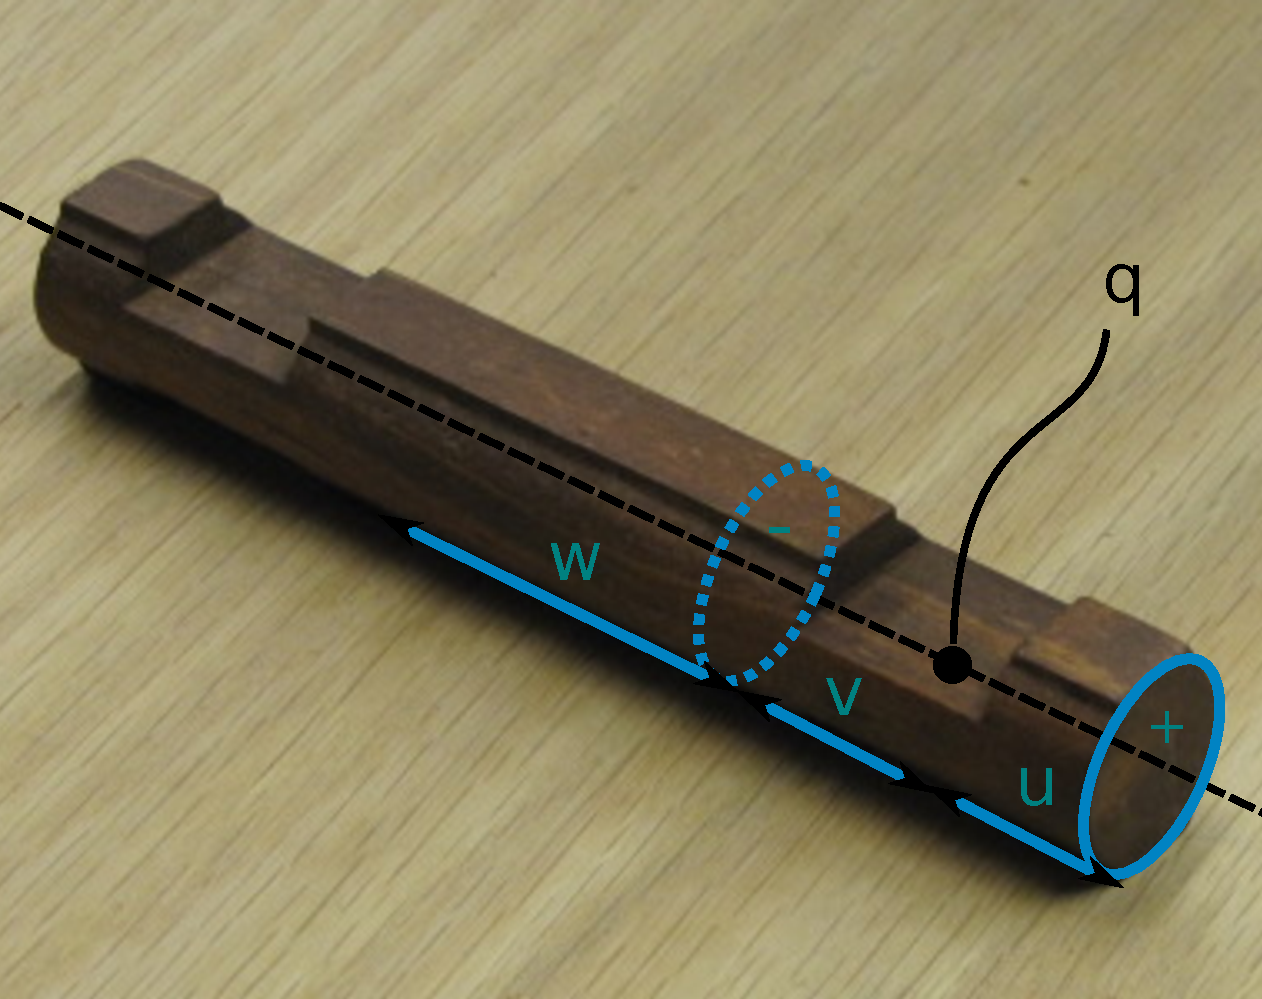
\includegraphics[width=0.47\textwidth]{images/real-log-qw}&
    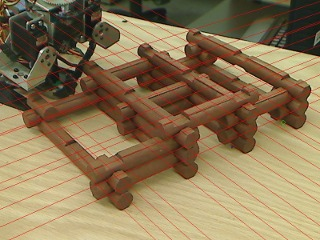
\includegraphics[width=0.493\textwidth]{images/pose2-cut}\\
    (a)&(c)
  \end{tabular}
  \vspace*{2ex}
  \begin{tabular}{@{}c@{\hspace{2pt}}c@{\hspace{2pt}}c@{\hspace{2pt}}c@{}}
    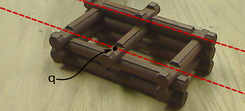
\includegraphics[width=0.24\textwidth]{images/poss-0-small}&
    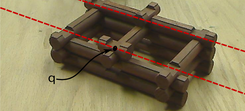
\includegraphics[width=0.24\textwidth]{images/poss-1-small}&
    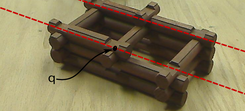
\includegraphics[width=0.24\textwidth]{images/poss-2-small}&
    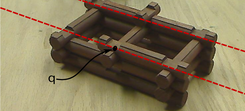
\includegraphics[width=0.24\textwidth]{images/poss-3-small}\\
    $\emptyset$&$(1,1)$&$(1,2)$&$(2,2)$\\[1ex]
    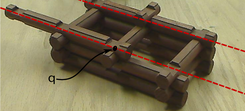
\includegraphics[width=0.24\textwidth]{images/poss-4-small}&
    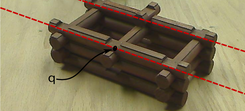
\includegraphics[width=0.24\textwidth]{images/poss-5-small}&
    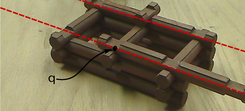
\includegraphics[width=0.24\textwidth]{images/poss-6-small}&\\
    $(1,3)$&$(2,3)$&$(3,3)$&\\
    \multicolumn{4}{c}{(b)}
  \end{tabular}
  %
  \par\vspace*{-2ex}
  %
  \caption{We generate two kinds of random variables for each grid
    position~$q$: log-feature variables~(a) that encode the observed image
    evidence for portions of logs and log-occupancy variables~(b) that encode
    the structure.
    %
    The overall process of structure estimation involves determining the
    unknown values of the log-occupancy variables~(b) from the observed image
    evidence represented through provided values of the log-feature
    variables~(a).
    %
    This process is mediated through the constraints shown in
    Figure~\protect\ref{fig:grammar-assemblies}(a).
    %
    (a)~The Boolean log-feature variables~$Z^+_q$, $Z^-_q$, $Z^u_q$, $Z^v_q$,
    and~$Z^w_q$ encode the presence of the specified image features for grid
    position~$q$.
    %
    (b)~The log-occupancy variable~$Z_q$ for grid position~$q$ takes one of
    a finite set of possible values: $\emptyset$~to denote that~$q$ is
    unoccupied and $(m,n)$ to denote occupancy by the~$m^{\textrm{th}}$ notch
    of an $n$-notch log.
    %
    (c)~Example of the underlying symbolic grid of a \LincolnLog\
    assembly.}
  %
  \label{fig:lincoln-logs}
  \par\vspace*{-2.5ex}
\end{figure}

This approach is demonstrated in the domain of \LincolnLogs, a children's
assembly toy with a small part inventory, namely, 1-, 2-, and 3-notch
logs.
%
In a grammatical \LincolnLog\ assembly, all logs lie on a symbolic grid imposed
over the structure (Figure~\ref{fig:lincoln-logs}c).
%
The structure of an assembly can be completely and unambiguously described by
specifying the occupancy at each grid position
(Figure~\ref{fig:lincoln-logs}b).
%
Not all possible occupancy descriptions denote stable, physically realizable
structures.
%
The space of valid structures can be specified by local constraints on the
occupancy of adjacent grid positions, as shown in
Figure~\ref{fig:grammar-assemblies}(a).
%
Enforcing these constraints over the entire structure renders some assemblies
grammatical and others ungrammatical, as shown in
Figure~\ref{fig:grammar-assemblies}(b).

\begin{figure}
  \centering
  \begin{tabular}{@{}l@{}}
    2-notch logs occupy 2 adjacent grid points\\
    3-notch logs occupy 3 adjacent grid points\\
    1- and 2-notch logs must be supported at all notches\\
    3-notch logs must be supported in at least 2 notches\\
    log ends must be at the ends of logs\\
    short segments indicate occupancy above or below\\
    long segments indicate presence of a multi-notch log\\[1ex]
    \multicolumn{1}{c}{(a)}
  \end{tabular}
  \par\vspace*{2ex}
  \begin{tabular}{@{}c@{\hspace{2pt}}c@{}}
    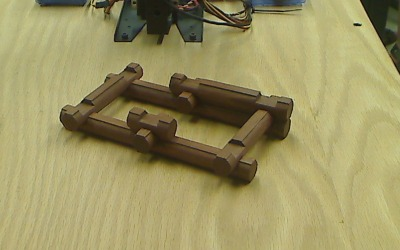
\includegraphics[width=0.48\textwidth]{images/valid-assemblies-1}&
    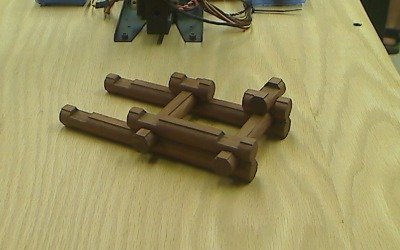
\includegraphics[width=0.48\textwidth]{images/valid-assemblies-2}\\[-0.5ex]
    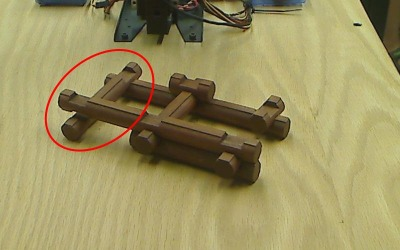
\includegraphics[width=0.48\textwidth]{images/invalid-assemblies-1}&
    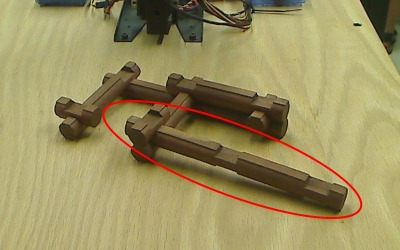
\includegraphics[width=0.48\textwidth]{images/invalid-assemblies-2}\\[1ex]
    \multicolumn{2}{c}{(b)}
  \end{tabular}
  %
  \par\vspace*{-2ex}
  %
  \caption{(a)~The constraints that encode the grammar of \LincolnLogs.
    %
    (b, top)~Examples of structures that satisfy the grammar.
    %
    (b, bottom)~Examples of structures that do not satisfy the grammar, because
    of unsupported logs.}
  %
  \label{fig:grammar-assemblies}
  %
  \par\vspace*{-3ex}
\end{figure}

\LincolnLogs, being cylindrical, generate two predominant image features:
\defoccur{log ends}, ellipses that result from the perspective projection of
circular log ends, and \defoccur{log segments}, line segments that result from
the perspective projection of cylindrical walls.
%
Boolean random variables~$Z^+$ and~$Z^-$ are constructed to encode the
presence of log-end features in the image.
%
Similar Boolean random variables~$Z^u$, $Z^v$, and~$Z^w$ are constructed
to encode the presence of log-segment features in the image.
%
There is one instance of each such variable, $Z^+_q$, $Z^-_q$, $Z^u_q$,
$Z^v_q$, and~$Z^w_q$, for each grid position~$q$, as shown in
Figure~\ref{fig:lincoln-logs}(a).
%
We also construct a discrete random variable~$Z_q$ for each grid position~$q$
that ranges over its possible occupancies in the structure, as shown in
Figure~\ref{fig:lincoln-logs}(b).
%
In the exposition below, we use~$\mathbf{Z}^+$, $\mathbf{Z}^-$, $\mathbf{Z}^u$,
$\mathbf{Z}^v$, $\mathbf{Z}^w$, and~$\mathbf{Z}$ to denote the collections of
the variables~$Z^+_q$, $Z^-_q$, $Z^u_q$, $Z^v_q$, $Z^w_q$, and~$Z_q$ for all
of the grid positions~$q$ in the problem at hand.

The values of the log-feature variables are determined directly from the image.
%
The values of the log-occupancy variables, however, cannot be directly observed.
%
The essence of structure estimation is to determine the values of the
log-occupancy variables.
%
This is done by formulating and solving a constraint satisfaction problem that
mutually constraints the log-feature and log-occupancy variables, using
Algorithm~\ref{alg:structure}.
%
The constraints are formalizations of the world knowledge in
Figure~\ref{fig:grammar-assemblies}(a).
%
Because the image evidence as encoded in the log-feature variables is noisy,
unreliable, and incomplete (due to occlusion), we cannot treat this as a
symbolic CSP and instead treat this as a stochastic CSP.
%
Within this stochastic framework, structure estimation is performed by
establishing priors over the random variables~$Z^+_q$, $Z^-_q$, $Z^u_q$,
$Z^v_q$, and~$Z^w_q$ that correspond to log features using image evidence and
establishing a uniform prior over the random variables~$Z_q$ that correspond to
the latent structure.
%
The random variables that correspond to log features are marginalized
\footnote{Marginalization is the process of deriving the joint distribution~$M$
  of a \emph{subset}, say~$\{A\}$, of the constituent variables of a joint
  distribution over all of the variables, say $\{A,B,C\}$.
  %
  We compute such as $M = \Pr\left(A\right) = \sum_{B,C} \Pr\left(A,B,C\right)$.
  %
  We utilize this in order to be able to derive the distribution over log
  occupancies, which is what we want, from the joint distribution over
  log occupancies and observed image evidence, which is what we have.
  %
  Historically, this term evolved from the practice of displaying the values of
  a joint distribution $\Pr(A,B)$ as a two-dimensional table with rows for
  the~$A$ entries and columns for the~$B$ entries.
  %
  The values of $\Pr(A)$ were derived by summing along the columns to yield a
  new row at the bottom \emph{margin} of the table.
  %
  The values of $\Pr(B)$ were derived by summing along the rows to yield a
  new column at the right \emph{margin} of the table.
  %
  This led to $\Pr(A)$ and $\Pr(B)$ being referred to as \emph{marginal}
  probabilities and the derivation process as \emph{marginalization}.}
and the resulting marginal distribution is conditioned on the language
model~$\Phi$ to enforce the constraints from
Figure~\ref{fig:grammar-assemblies}(a).
%
Finally, the assignment to the collection, $\mathbf{Z}$, of random
variables~$Z_q$, that maximizes this conditional marginal probability is
computed:

\par\vspace*{-2ex}
\begin{equation}
  \argmax_{\mathbf{Z}}\hspace{-13pt}
  \sum_{\substack{\mathbf{Z}^+,\mathbf{Z}^-,\mathbf{Z}^u,\mathbf{Z}^v,\mathbf{Z}^w\\
      \Phi\left[\mathbf{Z},\mathbf{Z}^+,\mathbf{Z}^-,\mathbf{Z}^u,\mathbf{Z}^v,\mathbf{Z}^w\right]}}
  \hspace{-10pt}\Pr\left(\mathbf{Z},\mathbf{Z}^{+},\mathbf{Z}^{-},\mathbf{Z}^u,\mathbf{Z}^v,\mathbf{Z}^w\right)
  \label{eq:structure-estimation}
\end{equation}
%
While this method can determine the conditional probability distribution over
consistent structures given image evidence, doing so is combinatorially
intractable.
%
To see why this is so, consider a simple $2 \times 2 \times 2$ grid
representing the underlying structure of a hypothetical \LincolnLog\ assembly.
%
Even for so small an assembly, since each grid position can take one of seven
possible values, the total number of possibilities ($7^8 \approx 5 \times
10^6$), exponential in the number of grid points, is huge.
%
This is due to the generative nature of the \LincolnLog\ domain.
%
We illustrate this point further with Figure~\ref{fig:complexity}(c), where we
enumerate the number of possible structures and how many of such are valid
given our system of constraints, for a few relatively small grid sizes.

\begin{figure}
  \centering
  \begin{tabular}{@{}c@{\hspace*{2pt}}c@{}}
    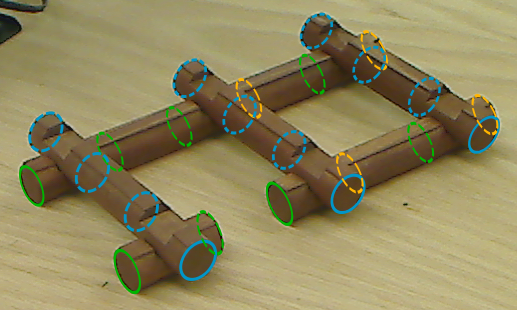
\includegraphics[width=0.45\textwidth]{images/log-end-visibility}&
    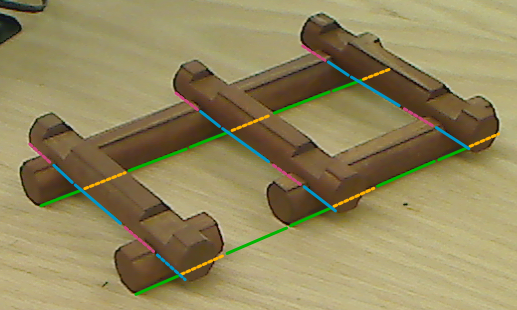
\includegraphics[width=0.45\textwidth]{images/log-segment-visibility}\\
    (a)&(b)
  \end{tabular}
  \par\vspace*{1ex}
  \begin{tabular}{@{}rc@{}}
    \raisebox{15ex}{(c)}&
    \begin{tabular}[b]{@{}c@{\hspace{10pt}}r@{\hspace{10pt}}r@{\hspace{10pt}}r@{}}
      \toprule
      $\substack{\text{\normalsize size}\\[0.5ex]
        \left(\text{X} \times \text{YX} \times \text{YZ} \times \text{Z}\right)}$ &
      \# grid points &
      $\substack{\text{\normalsize possible}\\ \text{\normalsize structures}}$ &
      $\substack{\text{\normalsize valid}\\ \text{\normalsize structures}}$\\[1ex]
      \midrule
      $2 \times 2 \times 2 \times 2$ &           $8$ & $5 \times 10^{6}$ &    $233$\\
      $2 \times 3 \times 2 \times 2$ &          $12$ &         $10^{10}$ &   $1341$\\
      $2 \times 3 \times 3 \times 2$ &          $16$ &         $10^{13}$ &   $6667$\\
      $3 \times 2 \times 2 \times 3$ &          $12$ &         $10^{10}$ &   $5461$\\
      $3 \times 2 \times 2 \times 3$ &          $18$ &         $10^{15}$ & $670179$\\
      \bottomrule
    \end{tabular}\\
    \raisebox{15ex}{(d)} & 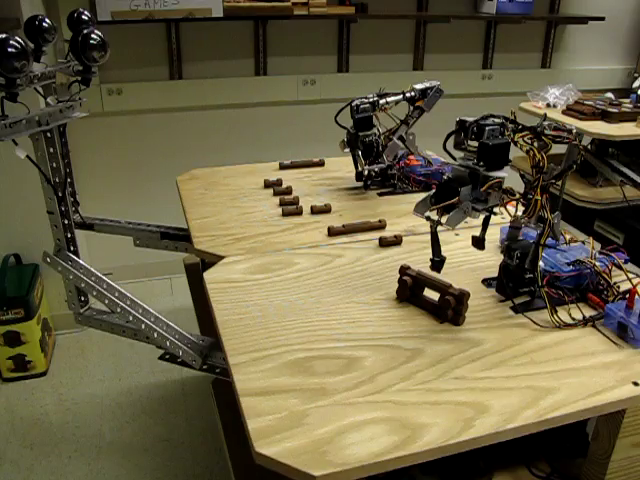
\includegraphics[width=0.55\textwidth]{images/robots}
  \end{tabular}
  %
  \par\vspace*{-2ex}
  %
  \caption{Example visibility estimates for (a)~log ends and (b)~log segments.
    %
    Green and orange indicate the visible and occluded features for
    even layers, while blue and magenta indicate visible and occluded features
    for odd layers.
    %
    (c)~Size of the space of \LincolnLog\ assemblies for given grid
    sizes.
    %
    $XZ$~is the ground plane while~$YX$ and~$YZ$ are the heights of the
    assembly along the respective ground-plane axes.
    %
    (d)~Our robotic environment for performing structure estimation
    with a rotating head to image the assembly from different viewpoints and a
    robot arm to disassemble the assembly.}
  %
  \label{fig:complexity}
  %
  \par\vspace*{-5ex}
\end{figure}

\begin{algorithm}[t]
  \caption{The structure-estimation algorithm as described in
    Section~\ref{sec:structure}.}
  %
  \SetKwData{Feature}{log-feature}
  \SetKwData{Features}{log-features}
  \SetKwData{GridPositions}{grid-positions}
  \SetKwData{GridPosition}{grid-position}
  \SetKwData{Grid}{grid}
  \SetKwData{BestP}{best-probability}
  \SetKwData{BestS}{best-structure}
  \SetKwData{Pro}{probability}
  \SetKwData{Image}{image}
  \SetKwData{Constraints}{constraints}
  \SetKwFunction{Uniform}{uniform}
  \SetKwFunction{Detector}{detector}
  \SetKwFunction{Nonempty}{nonempty}
  \SetKwFunction{Bound}{bound}
  \SetKwFunction{Probability}{Pr}
  \SetKwFunction{Backtrack}{backtrack}
  \SetKwFunction{Bind}{bind}
  \SetKwFunction{Unbound}{unbound}
  \SetKwFunction{Bound}{bound}
  \SetKwFunction{Select}{select}
  \SetKwFunction{AC}{arc-consistency}
  \SetKwFunction{CSPSolutionsExist}{csp-solutions-exist}
  \SetKwFunction{Inconsistent}{inconsistent}
  \GridPositions$\leftarrow$ $(\forall_{\GridPosition\in\Grid})$
  \Uniform{$\{\emptyset,(1,1),(1,2),(2,2),(1,3),(2,3),(3,3)\}$}\;
  \Features$\leftarrow$ $(\forall_{\Feature\in\Grid})$
  \Detector{\Feature,\Image}\;
  \BestP$\leftarrow-\infty$\;
  \While{\CSPSolutionsExist{}}{
    \Pro$\leftarrow$\hspace{-5ex}$\displaystyle \prod_{\Bound{\Features}}$\hspace{-5ex}
    \Probability{\Feature}\hspace{-5ex}$\displaystyle
    \prod_{\Bound{\GridPositions}}$ \hspace{-5ex}\Probability{\GridPosition}\;
    \If{$(\forall_{\Features})$\Bound{\Feature}$\wedge$
      $(\forall_{\GridPositions})$\Bound{\GridPosition}}{
      \If{\Pro$>$ \BestP}{\BestP$\leftarrow$ \Pro\;
        \BestS$\leftarrow$ \GridPositions\;
      }
      \Backtrack{}\;
    }
    \lIf{\Pro$<$ \BestP}{\Backtrack{}}\;
    \Bind{\Select{\Unbound{\GridPosition$\cup$ \Feature}}}\;
    \AC{\Constraints}\;
    \lIf{\Inconsistent{}}{\Backtrack{}}
  }
  \label{alg:structure}
\end{algorithm}

To compute Equation~\ref{eq:structure-estimation}, we employ algorithms
for each of the constituent processes that help ameliorate this intractability.
%
These algorithms prune the space so as not to enumerate all possible
structures, and hence cannot obtain the distribution over structures.
%
The conditional marginalization process is made tractable by pruning
assignments to the random variables that violate the grammar~$\Phi$ using arc
consistency \cite{Mackworth1977}.
%
The maximization process is made tractable by using a branch-and-bound
algorithm \cite{Land1960} that maintains upper and lower bounds on the maximal
conditional marginal probability.
%
Instead of determining the distribution over structures, this yields a single
most-likely consistent structure given the image evidence, along with its
probability.
%
Algorithm~\ref{alg:structure} gives pseudo-code for the structure-estimation
process.

\par\vspace{-1ex}
\section{Visibility Estimation}
\label{sec:visibility}

Image evidence for the presence or absence of each log feature is obtained
independently.
%
Each log feature corresponds to a unique local image property when projected to
the image plane under the known camera-relative pose.
%
A prior over the random variable associated with a specific log feature can be
determined with a detector that is focused on the expected location and shape
of that feature in the image given the projection.
%
This assumes that the specific log feature is visible in the image, and not
occluded by portions of the assembly between the camera and that log feature.
%
We show example visibility of log-end and log-segment features for a simple
\LincolnLog\ assembly in Figure~\ref{fig:complexity}(a,b).
%
When the log feature~$f$, a member of the set $\{+,-,u,v,w\}$ of the five
feature classes defined above, at a position~$q$, is not visible, the prior can
be taken as uniform, allowing the grammar to fill in unknown information.
%
We represent the visibility of a feature~$f$ at position~$q$ by the boolean
variable~$V^f_q$, where:

\par\vspace*{-4ex}
\begin{subequations}
  \begin{align}
    &\Pr(Z^f_q=\true)\propto\text{image evidence}&\text{when $V^f_q=\true$}\\[-1ex]
    &\Pr(Z^f_q=\false)=\frac{1}{2}&\text{otherwise.}
  \end{align}
  \label{eq:visibility}
  \vspace*{-2ex}
\end{subequations}

\par\vspace*{-1ex}\noindent
In order to do so, it is necessary to know which log features are visible and
which are occluded so that image evidence is only applied to construct a prior
on visible log features, using Equation~\ref{eq:visibility}(a), and a uniform
prior is constructed for occluded log features, using
Equation~\ref{eq:visibility}(b).
%
Thus, in Rumsfeld's terminology, one needs to know the known unknowns in order
to determine the unknowns.
%
This creates a chicken-and-egg problem.
%
To determine whether a particular log feature is visible, one must know the
composition of the structure between that feature and the camera.
%
Likewise, to determine the structure composition, one must know which log
features are visible.
%
While earlier work \cite{Siddharth2011} demonstrated successful automatic
determination of log occupancy at occluded log positions, it could only do so
given manual annotation of log-feature visibility.
%
In other words, while~$Z_q$ was automatically inferred, it required manual
annotation of~$V^f_q$.
%
Further, manual annotation of~$V^f_q$ required implicit human awareness
of~$Z_q$.

We extend this prior work to automatically determine visibility of log features
in tandem with log occupancy.
%
Our novel contribution in this section is mutual automatic determination of
both~$Z_q$ and~$V^f_q$ solving the chicken-and-egg problem inherent in doing so
with an iterative algorithm reminiscent of expectation maximization
\cite{DempsterLR77}.
%
We start with an initial estimate of the visibility of each log feature.
%
We apply the structure-estimation procedure to estimate the occupancy of each
symbolic grid position and use the estimated structure to recompute a new
estimate of log-feature visibility and iterate this process until a fixpoint is
reached.
%
There are two crucial components in this process: determining the initial
log-feature visibility estimate and reestimating log-feature visibility from an
estimate of structure.

We determine the initial log-feature visibility estimate, $V^f_q$, by assuming
that the structure is a rectangular prism whose top face and two camera-facing
front faces are completely visible, and whose other faces are not.
%
No assumptions are made about the constituents of the structure, its pose, or
the camera views used.
%
We use the camera-relative pose of the symbolic grid (which can be determined
without any knowledge of the structure) together with the maximal extent of
each of the three symbolic grid axes, three small integers which are currently
specified manually, to determine the visible faces.
%
We determine the image positions for four corners of the base of this
rectangular prism and the bottommost three such image positions as they
correspond to the endpoints of the lower edges of the two frontal faces.
%
It is possible that one of these faces is nearly parallel to the
camera axis and thus invisible.
%
We determine that this is the case when the angle subtended by the two lower
edges is less than 110$^{\circ}$ and discard the face whose lower edge has
minimal image width.
%
This process does nothing more than establish that, in the absence of a
structure estimate from which to derive visibility, the front and top faces of
the grid are the only parts for which the log-feature random variables have
image evidence as their support, using Equation~\ref{eq:visibility}(a).
%
All other parts of the grid are taken to have the uniform distribution as their
support, using Equation~\ref{eq:visibility}(b), as a means of saying that we
assume nothing about them.

We update the log-feature visibility estimate from a structure estimate by
rendering the structure in the context of the known camera-relative pose of the
symbolic grid.
%
We characterize each log feature with a fixed number of points, equally spaced
around circular log ends or along linear log segments and trace a ray from each
such point's 3D position to the camera center, asking whether that ray
intersects some bounding cylinder for a log in the estimated structure.
%
We take a log feature to be occluded when 60\% or more of such rays intersect
logs in the estimated structure.
%
Structure estimation isn't adversely affected by a moderate number of log
features incorrectly labeled as occluded because it can use the grammar to
determine occupancy of the corresponding grid positions.

\begin{algorithm}[t]
  \caption{The visibility-estimation algorithm as described in
    Section~\ref{sec:visibility}, using Algorithm~\ref{alg:structure}.}
  %
  \SetKwData{Feature}{log-feature}
  \SetKwData{Features}{log-features}
  \SetKwData{Visible}{visible}
  \SetKwData{Grid}{grid}
  \SetKwData{PreviousStructure}{previous-structure}
  \SetKwData{CurrentStructure}{current-structure}
  \SetKwData{RenderedImage}{rendered-image}
  \SetKwFunction{RenderStructure}{render-structure}
  \SetKwFunction{SE}{structure-estimation}
  \SetKwFunction{IsVisible}{is-visible}
  \Visible$\leftarrow$ \emph{top and front of structure}\;
  \CurrentStructure$\leftarrow$ $\emptyset$\;
  \Repeat{\PreviousStructure $=$ \CurrentStructure}{
    \PreviousStructure$\leftarrow$ \CurrentStructure\;
    \CurrentStructure$\leftarrow$ \SE{$(\forall_{\Feature \notin \Visible})\Pr(\Feature) = \frac{1}{2}$}\;
    \Visible$\leftarrow$ $\emptyset$\;
    \RenderedImage$\leftarrow$ \RenderStructure{\CurrentStructure}\;
    \ForAll{\Features$\in$ \Grid}{
      \lIf{\IsVisible{\Feature, \RenderedImage}}{\Visible $\leftarrow$
        \Visible $\cup$ $\{\Feature\}$
      }
    }
  }
  \label{alg:visbility}
\end{algorithm}

We perform such rendering efficiently by rasterization.
%
We begin with an empty bitmap, iterate over each log feature and each occupied
grid position that lies between that log feature and the camera center, and
render a projection of the bounding cylinder of the log at that grid position
on the bitmap.
%
This renders all possible occluders for each log feature, allowing one to
determine visibility by counting the rendered pixels at points that correspond
to the projected rays.

The above process might not reach a fixpoint and instead enter an infinite loop
of pairs of visibility and structure estimates.
%
In practice, this process reaches a fixpoint or enters a short loop within
three to four iterations, making loop detection straightforward.
%
When a loop is detected, we select the structure in the loop with the highest
probability estimate.
%
Algorithm~\ref{alg:visbility} provides the pseudo-code that summarizes the
above process.

\par\vspace{-1ex}
\section{Structure-Estimation Confidence}
\label{sec:confidence}

While the structure-estimation process can determine the occupancy of a small
number of grid positions when only a single set of occupancy values is
consistent with the grammar and the image evidence, it is not clairvoyant; it
cannot determine the structure of an assembly when a large part of that
assembly is occluded and many different possible structures are consistent with
the image evidence.
%
In this case, we again have an issue of unknowns \vs\ known unknowns: how can
one determine one's confidence in one's structure estimation?
%
If we could determine the conditional distribution over consistent structures
given image evidence, $\Pr(\mathbf{Z}|I)$, a measure of confidence could be
entropy of this distribution, $H(\mathbf{Z}|I)$.
%
However, as discussed previously, computing this distribution is intractable
and consequently so is computing its entropy.\footnote{The entropy $H(Z)$ of a
  random variable~$Z$ is $\sum_{z\in Z}\Pr(z)\log\Pr(z)$.
  %
  It measures the information content of a random variable, or lack thereof.
  %
  Computing this requires summing over all elements in~$Z$.}
%
Thus we adopt an alternate means of measuring confidence in the result of the
structure-estimation process.

Given a visibility estimate, $V^f_q$, structure estimate, $\mathbf{Z}$, and
priors on random variables associated with log features computed with
image evidence, $Z^f_q$, one can marginalize over the random variables
associated with visible log features and compute the maximum-likelihood
assignment to the random variables associated with occluded log features,
$\hat{\mathbf{Z}}^f$, consistent with a given structure estimate:
%
\begin{equation*}
  \hat{\mathbf{Z}}^f=
  \argmax_{\substack{Z^f_q\\V^f_q=\false}}\hspace{-4.5ex}
  \sum_{\substack{Z^f_q\\V^f_q=\true\\
      \Phi[\mathbf{Z},\mathbf{Z}^{+},\mathbf{Z}^{-},\mathbf{Z}^u,\mathbf{Z}^v,\mathbf{Z}^w]}}\hspace{-6ex}
  \Pr(\mathbf{Z},\mathbf{Z}^{+},\mathbf{Z}^{-},\mathbf{Z}^u,\mathbf{Z}^v,\mathbf{Z}^w)
\end{equation*}
%
One can then ask the following question: what is the maximal amount~$\delta$
that one can shift the probability mass on the occluded log-feature random
variables \emph{away} from the uniform prior, reassigning it to the opposite
element of its support, such that estimated structure remains the same?
%
Or in simpler terms: \emph{Assume an initial structure estimate derived from a
  uniform prior over occluded log features.
  %
  How much hypothetical evidence for such features is needed to change my mind
  about the structure?}
%
We compute~$\delta$ using a modified structure-estimation step:
%
\begin{equation*}
  \argmax_{\mathbf{Z}}\hspace{-5ex}
  \sum_{\substack{\mathbf{Z}^{+},\mathbf{Z}^{-},\mathbf{Z}^u,\mathbf{Z}^v,\mathbf{Z}^w\\
      \Phi[\mathbf{Z},\mathbf{Z}^{+},\mathbf{Z}^{-},\mathbf{Z}^u,\mathbf{Z}^v,\mathbf{Z}^w]}}\hspace{-5ex}
  \Pr(\mathbf{Z},\mathbf{Z}^{+},\mathbf{Z}^{-},\mathbf{Z}^u,\mathbf{Z}^v\,\mathbf{Z}^w)=\mathbf{Z}
\end{equation*}
%
when, for all $q^f$ where $V^f_q=\false$,
%
\begin{math}
    \Pr(Z^f_q=\neg\hat{Z}^f_q)=\frac{1}{2}+\delta
\end{math}
and
\begin{math}
    \Pr(Z^f_q=\hat{Z}^f_q)=\frac{1}{2}-\delta.
\end{math}
%
We call such a~$\delta$ the \defoccur{estimation tolerance}.
%
Then, for any estimated structure, one can make a confidence judgment by
comparing the estimation tolerance to an overall tolerance threshold~$\delta^*$.
%
One wishes to select a value for~$\delta^*$ that appropriately trades off false
positives and false negatives in such confidence judgments: we want to
minimize the cases that result in a positive confidence assessment for an
incorrect structure estimate and also minimize the cases that result in a
negative confidence assessment for a correct structure estimate.
%
Because the methods we present in the next section can gather additional
evidence in light of negative confidence assessment in structure estimation,
the former are more hazardous than the latter because they preclude gathering
additional evidence and lead to an incorrect structure estimate while the
latter simply incur the cost of additional evidence gathering.
%
Because of this asymmetry, our method is largely insensitive to the particular
value of~$\delta^*$ so long as it is sufficiently high to not yield excessive
false positives.

One can determine the estimation tolerance by binary search for the smallest
value of $\delta\in(0,0.5)$ that results in a different estimated structure, a
time-consuming process.
%
But we don't actually need the value of~$\delta$; we only need to determine
whether $\delta<\delta^*$.
%
We do this by simply asking whether the estimated structure, $\mathbf{Z}$,
changes when the probabilities are shifted by~$\delta^*$, \ie\
%
\begin{math}
    \Pr(Z^f_q=\neg\hat{Z}^f_q)=\frac{1}{2}+\delta^{*}
\end{math}
and
\begin{math}
    \Pr(Z^f_q=\hat{Z}^f_q)=\frac{1}{2}-\delta^{*}
\end{math}.
%
This involves only a single new structure estimation.
%
Initializing the branch-and-bound structure-estimation algorithm with the
probability of the original structure estimate given the modified distributions
for the random variables associated with occluded log features speeds this
process up.

\par\vspace{-1ex}
\section{Gathering Additional Evidence}
\label{sec:integration}

Structure estimation can be made more reliable by integrating multiple sources
of image evidence.
%
We perform structure estimation in a robotic environment, illustrated in
Figure~\ref{fig:complexity}(d), that facilities automatically gathering
multiple sources of image evidence as needed.
%
This workspace is imaged by a camera mounted on a pendulum arm that can rotate
180$^{\circ}$ about the workspace, under computer control, to image the
assembly from different viewpoints.
%
This can be used to view portions of the assembly that would otherwise be
occluded.
%
Moreover, a robotic arm can disassemble a structure on the workspace to reveal
the lower layers of a structure that would otherwise be occluded by higher
layers.
%
These methods can further be combined.
%
Generally speaking, we seek a method for constraining a single estimate
of an initial structure with multiple log features derived from different
viewpoints and different stages of disassembly.

We can do this as follows.
%
Let~$\mathbf{Z}$ be a collection of random variables~$Z_q$ associated with log
occupancy for a given initial structure.
%
Given multiple views $i=1,\ldots,n$ with collections~$\mathbf{Z}_i$ of random
variables~$Z^+_q$, $Z^-_q$, $Z^u_q$, $Z^v_q$, and~$Z^w_q$ associated with the
image evidence for log features from those views, we can compute:
%
\begin{equation*}
  \argmax_{\mathbf{Z}}\hspace{-12pt}
  \sum_{\substack{\mathbf{Z}_1\ldots\mathbf{Z}_n\\
      \Phi\left[\mathbf{Z},\mathbf{Z}_1\right]\wedge\cdots\wedge\Phi\left[\mathbf{Z},\mathbf{Z}_n\right]}}
  \hspace{-10pt}\Pr\left(\mathbf{Z},\mathbf{Z}_1,\ldots,\mathbf{Z}_n\right)
\end{equation*}
%
Two issues arise in doing this.
%
First, though one can estimate the camera-relative pose of the structure
independently for each view, this does not yield the registration between these
views.
%
There are only four possible symbolic orientations of the structure in each
view so for~$n$ views we need only consider~$4^{n-1}$ possible combinations.
%
We can greedily search for the combination that yields the maximum-likelihood
structure estimate by incrementally adding views to the structure-estimation
process and registering each added view by searching for the best among the
four possible registrations.
%
Second, in the case of partial disassembly, we need to handle the fact that the
partially disassembled structure is a proper subset of the initial structure.
%
We do this by omitting random variables associated with log features
for logs that are known to have been removed in the disassembly process and not
instantiating constraints that mention such omitted random variables.

We can combine the techniques from Section~\ref{sec:confidence} with these
techniques to yield an active-vision \cite{Bajcsy1988} approach to producing a
confident and correct structure estimate.
%
One can perform structure estimation on an initial image and assess one's
confidence in that estimate.
%
If one is not confident, one can plan a new observation, entailing either a new
viewpoint, a partial-disassembly operation, or a combination of the two and
repeat this process until one is sufficiently confident in the estimated
structure.
%
We plan new observations by asking the following question: which of the
available actions maximally increases confidence?
%
Like before, if we could determine the conditional distribution over consistent
structures given image evidence, we could select the action which maximally
decreases entropy.
%
But again, neither computing this distribution nor consequently computing its
entropy is tractable, as discussed previously.
%
Thus we adopt an alternate means of measuring increase in confidence.

Consider view~$i$ of the~$n$ current views.
%
For such~$i$, consider the given visibility estimates $V^f_{iq}$, priors
$Z^f_{iq}$ on the log-feature random variables computed with image evidence,
and a structure estimate~$\mathbf{Z}$ constructed from such views.
%
We can marginalize over random variables associated with visible log features
$V^f_{iq} = \true$ and compute the maximum-likelihood assignment
$\hat{\mathbf{Z}}^f$ to the random variables associated with occluded log
features that is consistent with a given structure estimate:
%
\begin{equation*}
  \hat{\mathbf{Z}}^f=\argmax_{\substack{Z^f_{iq},V^f_{iq}=\false}}
  \sum_{\substack{Z^f_{iq},V^f_{iq}=\true\\
      \Phi[\mathbf{Z},\mathbf{Z}_1]\wedge\cdots\wedge\Phi[\mathbf{Z},\mathbf{Z}_n]}}
  \Pr(\mathbf{Z},\mathbf{Z}_1,\ldots,\mathbf{Z}_n)
\end{equation*}
%
We determine those log features that are invisible in all current views but
visible in a new view resulting from a hypothetical action.
%
One can then ask the following question: what is the maximal amount~$\delta'$
that one can shift the probability mass on these random variables \emph{away}
from the uniform prior, reassigning it to the opposite element of its support,
such that the estimated structure with the new view remains the same.
%
In simpler terms: \emph{Assume an initial structure estimate derived from a
  uniform prior over occluded log features.
  %
  Imagine a hypothetical action which renders such occluded log features
  visible.
  %
  For such an imagined view, how much hypothetical evidence for such log
  features, in all current views, is needed to change my mind about the
  structure?}

\par\noindent
%
For an action yielding a new view, $j$, we compute $\delta'$ as
%
\begin{equation*}
  \argmax_{\mathbf{Z}}\hspace{-5ex}
  \sum_{\substack{\mathbf{Z}_1\ldots\mathbf{Z}_n\;\mathbf{Z}_j\\
      \Phi[\mathbf{Z},\mathbf{Z}_1]\wedge\cdots\wedge\Phi[\mathbf{Z},\mathbf{Z}_n]
      \wedge\Phi[\mathbf{Z},\mathbf{Z}_j]}}\hspace{-6ex}
  \Pr(\mathbf{Z},\mathbf{Z}_1,\ldots,\mathbf{Z}_n,\mathbf{Z}_j)=\mathbf{Z}
\end{equation*}
when
\begin{math}
    \Pr(Z^f_{iq}=\neg\hat{Z}^f_{iq})=\frac{1}{2}+\delta
\end{math}
and
\begin{math}
    \Pr(Z^f_{iq}=\hat{Z}^f_{iq})=\frac{1}{2}-\delta
\end{math}
$\forall q^f:V^f_{jq}=\true\wedge(\forall i)V^f_{iq}=\false$.
%
We perform binary search to find~$\delta'$ for each hypothetical action
and select the one with the lowest~$\delta'$.
%
This nominally requires sufficiently deep binary search to compute~$\delta'$ to
arbitrary precision.
%
One can make this process faster by performing binary search on all
hypothetical actions simultaneously and terminating when there is only one
action lower than the branch point.
%
This requires that binary search be only sufficiently deep to discriminate
between the available actions.

\par\vspace{-1ex}
\section{Natural Language}
\label{sec:language}

An interesting feature of our framework is that it allows for elegant inclusion
of information from other modalities.
%
Natural language, for example, can be integrated into our approach to draw
additional evidence for structure estimation from utterances describing the
structure in question.
%
A sentence, or set of sentences, describing a structure need not specify the
structure unambiguously.
%
Much like additional images from novel viewpoints can provide supplementary but
partial evidence for structure estimation, sentences providing incomplete
descriptions of structural features also can provide supplementary but partial
evidence for structure estimation.

We have investigated this possibility via a small domain-specific language for
describing some common features present in assembly toys.
%
This language has: three nouns (\emph{wall}, \emph{window}, and \emph{door}),
four spatial relations (\emph{left of}, \emph{right of}, \emph{perpendicular
  to}, and \emph{coplanar to}), and one conjunction (\emph{and}).
%
Sentences constructed from these words can easily be parsed into logical
formulas.

Analogous to how a CSP encodes the validity of an assembly through a set of
constraints, such logical formulas derived from sentential descriptions can also
constrain the structures to be considered.
%
The words in our vocabulary impose the following constraints:
%
\vspace*{0.9ex}
\begin{compactenum}
\item A \emph{wall} is composed of a rectangular vertical coplanar set of grid
  points.
  %
  All grid points in the wall must be occupied.
\item A \emph{door} is composed of a rectangular vertical coplanar set of grid
  points.
  %
  All grid points inside the door must be unoccupied.
  %
  All grid points on the door posts must be log ends facing away from the door.
  %
  All grid points on the mantel must be occupied by the same log.
  %
  The threshold must be unoccupied and at the bottom of the structure.
\item A \emph{window} is similar to a door whose threshold is occupied by the
  same log and is not constrained to be at the bottom of the structure.
\item \emph{Perpendicular to} constrains the grid points of two
  entities to lie on perpendicular axes.
  %
  \emph{Coplanar to} is analogous.
\item \emph{Right of} or \emph{left of} constrain the relative coordinates of
  the grid points of two entities.
\end{compactenum}
\vspace*{0.9ex}

\par\noindent
We have given formal semantic definitions for $8$ words in terms of CSP
fragments.
%
These are defined informally in English above.
%
We omit the formal definitions since they are tedious.
%
Nonetheless, our implementation parses sentences containing these words and
applies the rules of compositional semantics to derive an overall CSP that
reflects the semantics of the sentence, from the CSP fragments that reflect the
semantics of the individual words.
%
This CSP which encodes constraints derived from natural language is then
combined with the CSPs which encode constraints derived from the visual
language model to perform structure estimation.
%
We thus compute a joint multiple-view and natural-language structure estimate
as follows.
%
Let~$\mathbf{Z}$ be a collection of random variables~$Z_q$ associated with log
occupancy for a given initial structure.
%
Given the set of constraints~$\Psi$ derived from natural language
and multiple views $i=1,\ldots,n$ with collections~$\mathbf{Z}_i$ of random
variables~$Z^+_q$, $Z^-_q$, $Z^u_q$, $Z^v_q$, and~$Z^w_q$ associated with the
image evidence for log features from those views, we compute
%
\begin{equation*}
  \argmax_{\mathbf{Z}}\hspace{-12pt}
  \sum_{\substack{\mathbf{Z}_1\ldots\mathbf{Z}_n\\
      \Phi\left[\mathbf{Z},\mathbf{Z}_1\right]\wedge\cdots\wedge\Phi\left[\mathbf{Z},\mathbf{Z}_n\right]\wedge\Psi\left[\mathbf{Z}\right]}}
  \hspace{-10pt}\Pr\left(\mathbf{Z},\mathbf{Z}_1,\ldots,\mathbf{Z}_n\right)
\end{equation*}
%
An example of how such an extension improves results is shown in
Figure~\ref{fig:language}.
%
The key idea here is that the CSP is a modality-neutral internal mental
representation that can be fed information derived by vision, language, or
both, allowing cross-modal inference.

A system that can accept and use such cross-modal information is in keeping
with our broader research effort to model human cognition.
%
All information that is available to the human brain is provided by means of
sensory input---eyes, ears, touch, \etc
%
To this effect, we fashion our systems to accept inputs with the same
modalities as humans; \ie\ raw camera input for vision, natural-language text
or speech for language, and motor-control primitives for proprioception.

\par\vspace{-1ex}
\section{Results}
\label{sec:results}

We gathered a corpus of five different images of each of~32 different structures,
each from a different viewpoint, for a total of~160 images.
%
The structures were carefully designed so that proper subset relations exist
among various pairs of the~32 distinct structures.

\begin{figure}
  \centering
  \begin{tabular}{@{}c@{}}
    \includegraphics[width=0.75\textwidth]{images/visibility}\\
    (a)\\
    \includegraphics[width=0.75\textwidth]{images/active-vision}\\
    (b)
  \end{tabular}
  %
  \par\vspace*{-2ex}
  %
  \caption{(a)~Error histograms for structure estimation with manual visibility
    annotation (in blue) and automatic visibility estimation (in red).
    %
    All of the structures estimated had 12 or fewer errors.
    %
    Note that the latter performs as well as the former.
    %
    (b)~Error histograms for the baseline structure estimation (in dark blue)
    and each of the active-vision process (partial disassembly in light blue,
    multiple views in yellow, and the combination of these in red).
    %
    Note that our active-vision processes consistently reduce estimation
    error.}
  %
  \label{fig:visibility}
  %
  \par\vspace*{-6ex}
\end{figure}

We first evaluated automatic visibility estimation.
%
We performed combined visibility and structure estimation on~105 of the~160
images and compared the maximum-likelihood structure estimate to that produced
by \singleemcite{Siddharth2011} using manual annotation of visibility.
%
For each image, we compare the maximum-likelihood structure estimate to ground
truth and compute the number of errors.
%
We do this as follows.
%
Each one-, two-, or three-notch log in either the ground truth or estimated structure
that is replaced with a different, possibly empty, collection of logs in the
alternate structure counts as a single error (which may be a deletion,
addition, or substitution).
%
Further, each collection of~$r$ adjacent logs with the same medial axis in
the ground truth that is replaced with a different collection of~$s$ logs in
the estimated structure counts as $\min(r,s)$ errors.
%
We then compute an error histogram of the number of images with fewer than~$t$
errors.
%
Figure~\ref{fig:visibility}(a)~shows the error histograms for manual visibility
annotation and automatic visibility estimation.
%
Note that the latter performs as well as the former---our automatic
visibility-estimation process appears to be reliable.

We then evaluated structure-estimation confidence assessment.
%
We computed the false-positive rate and false-negative rate of our
confidence-assessment procedure over the entire corpus of~105 images, where a
false positive occurs with a positive confidence assessment for an
incorrect structure estimate and a false negative occurs with negative
confidence assessment for a correct structure estimate.
%
This resulted in only three false positives and seven false negatives on our corpus.

\begin{figure}
  \centering
  \begin{tabular}{@{}c@{\hspace*{2pt}}c@{}}
    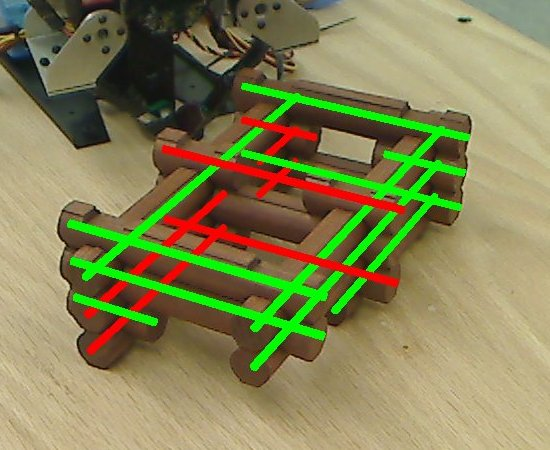
\includegraphics[width=0.48\textwidth]{images/cropped-1263242028-1800-a}&
    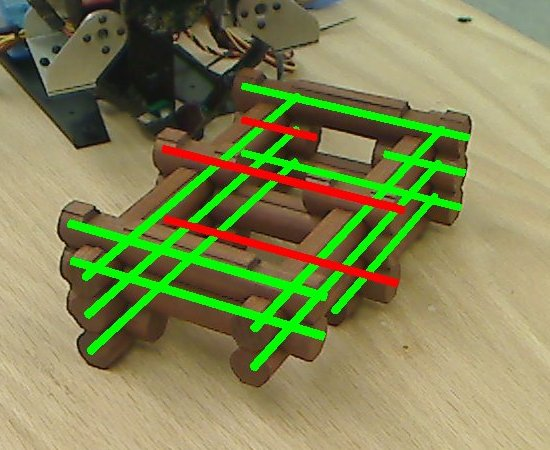
\includegraphics[width=0.48\textwidth]{images/cropped-1263242028-1800-b}\\
    (a)&(b)\\[1ex]
    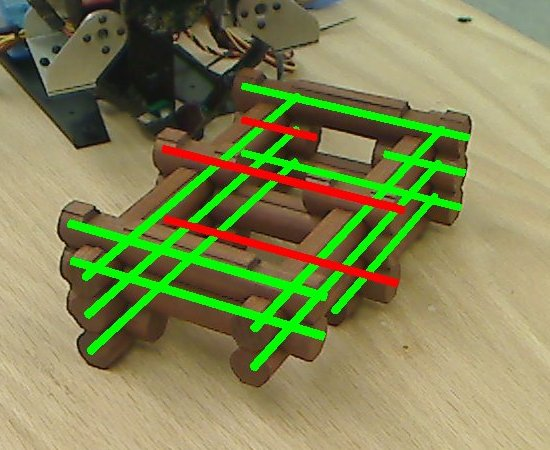
\includegraphics[width=0.48\textwidth]{images/cropped-1263242028-1800-c}&
    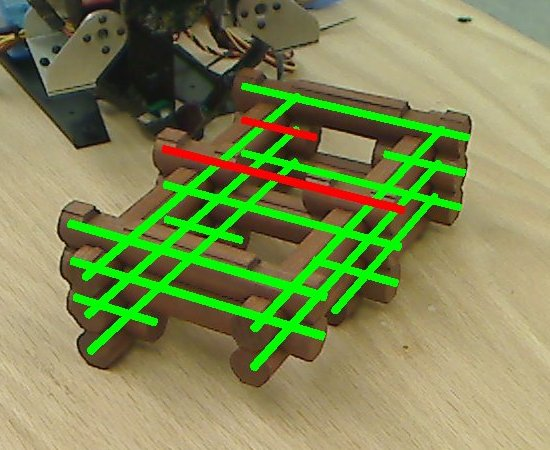
\includegraphics[width=0.48\textwidth]{images/cropped-1263242028-1800-d}\\
    (c)&(d)
  \end{tabular}
  %
  \caption{\small Estimated structure through the following four methods:
    %
    (a)~Baseline structure estimation.
    %
    (b)~Partial disassembly.
    %
    (c)~Multiple views.
    %
    (d)~Combined partial disassembly and multiple views.
    %
    Overlayed log color indicates correct (green) or incorrect (red)
    estimation of log occupancies.}
  %
  \label{fig:results}
  %
  \par\vspace*{-3ex}
\end{figure}

Next, we evaluated the active-vision process for performing requisite actions
to improve structure estimation confidence on~90 images from our corpus.
%
So as not to render this evaluation dependent on the mechanical reliability of
our robot (which is tangential to the current paper) and focus the evaluation on
the computational method, we use the fact that our corpus contains multiple
views of each structure from different viewpoints to simulate moving the robot
head to gather new views and the fact our corpus contains pairs of structures
in a proper-subset relation to simulate using the robot to perform partial
disassembly.
%
We first evaluated simulated robot-head motion to gather new views.
%
For each image, we took the other images of the same structure from different
viewpoints as potential actions and perform our active-vision process.
%
We next evaluated simulated robotic disassembly.
%
For each image, we took images of proper-subset structures taken from the same
viewpoint as potential actions and perform our active-vision process.
%
We finally evaluated simulated combined robot-head motion and robotic
disassembly.
%
For each image, we took all images of proper-subset structures taken from any
viewpoint as potential actions and perform our active-vision process.
%
For each of these, we computed the error histogram at the termination of the
active-vision process.
%
Figure~\ref{fig:visibility}(b)~shows the error histograms for each of the
active-vision processes together with the error histogram for baseline
structure estimation from a single view on this subset of~90 images.
%
Figure~\ref{fig:results} shows the final estimated structure when performing
each of the four processes from Figure~\ref{fig:visibility}(b)~on the same
initial image.
%
Note that our active-vision processes consistently reduce estimation error.

We demonstrate natural-language integration in Figure~\ref{fig:language}.
%
In (a), structure estimation is performed on a single view, which due to
occlusion, is unable to determine the correct structure.
%
A second view is acquired.
%
Note that this second view suffers from far more occlusion than the first view
and produces a far worse structure estimate (b).
%
The information available in these two views is integrated and jointly produces
a better structure estimate than either view by itself
(c).
%
However, this estimate is still imperfect.
%
To demonstrate the utility and power of integrating visual and linguistic
information, we intentionally discard the second view and construct an estimate
from just a single image, together with a single linguistic description, each of
which is ambiguous taken in isolation.
%
The user provides the sentence \emph{window left of and perpendicular to door}.
%
Note that this sentence does not fully describe the assembly.
%
It does not specify the number of windows and doors, their absolute
positions, or the contents of the rest of the structure.
%
Yet this sentence, together with the single image from the first view, is
sufficient to correctly estimate the structure (d).

\begin{figure}
  \centering
  \begin{tabular}{@{}c@{\hspace*{2pt}}c@{}}
    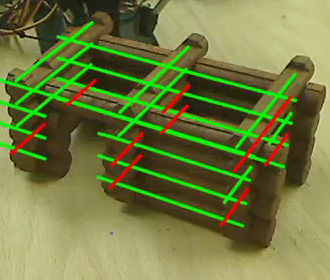
\includegraphics[width=0.48\textwidth]{images/language-view-one}&
    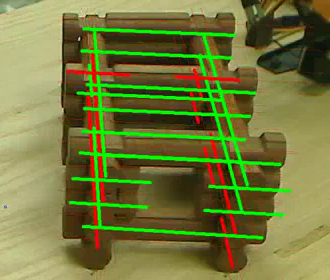
\includegraphics[width=0.48\textwidth]{images/language-view-two}\\
    (a) View $1$ & (b) View $2$\\[1ex]
    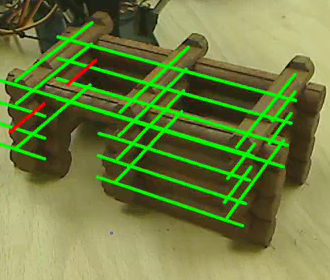
\includegraphics[width=0.48\textwidth]{images/language-view-one+two}&
    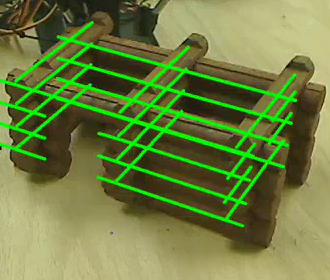
\includegraphics[width=0.48\textwidth]{images/language-view-one+sentence}\\
    (c) View $1 + 2$ & (d) View $1$ $+$ \emph{\textbf{Language}}
  \end{tabular}
  %
  \caption{\small An example of joint structure estimation from image evidence
    and natural language.
    %
    (a)~Structure estimation from an initial view.
    %
    (b)~Structure estimation from a second view alone.
    %
    (c)~Structure estimation using information from both views from the viewpoint of the first view.
    %
    (d)~Structure estimation integrating image evidence from the first view
    with the sentence \emph{\textbf{window left of and perpendicular to door}}.
    %
    Overlayed log color indicates correct (green) or incorrect (red) estimation
    of log occupancies.}
  %
  \label{fig:language}
  %
  \par\vspace*{-3ex}
\end{figure}

\par\vspace{-1ex}
\section{Related Work}
\label{sec:related}

Our work shares three overall objectives with prior work:
estimating 3D structure from 2D images, determining when there is
occlusion, and active vision.
%
However, our work explores each of these issues from a novel perspective.

Prior work on structure estimation (\eg\ \npcite{Saxena2007,Lee2009,Gupta2010})
focuses on \emph{surface estimation}, recovering 3D surface from 2D images.
%
In contrast, our work focuses on recovering the \emph{constituent structure}
of an assembly: what parts are used to make the assembly and how such parts are
combined.
%
Existing state-of-the-art surface reconstruction methods (\eg\ Make3D,
\npcite{Saxena2008} ) are unable to determine surface structure of the kinds of
\LincolnLog\ assemblies considered here.
%
Even if such surface estimates were successful, they are insufficient to
determine the constituent structure.

Prior work on occlusion determination (\eg\ \npcite{Gupta2010,Hoiem2011})
focuses on finding occlusion boundaries; the 2D image boundaries of occluded
regions, and estimating occlusion of object surfaces (\eg\
\npcite{bohg2011,moesenlechner11}) in $3$D using shape priors and symmetries.
%
In contrast, our work focuses on determining occluded \emph{parts} in the
constituent structure.
%
We see no easy way to determine occluded parts either from occlusion boundaries
or from occluded surfaces since such alone are insufficient to determine even
the number of occluded parts, let alone their types and positions in a 3D
structure.

Prior work on active vision (\eg\ \npcite{Maver1993}) focuses on integrating
multiple views into surface estimation and selecting new viewpoints to
facilitate such in the presence of occlusion.
%
In contrast, our work focuses on determining the confidence of constituent
structure estimates and choosing an action with maximal anticipated increase in
confidence.
%
We consider not only view changes but also robotic disassembly to view object
interiors.
%
Also note that the confidence estimates used in our approach are mediated by
the visual language model.
%
We might not need to perform active vision to observe all occluded structure as
it might be possible to infer part of the occluded structure.
%
Prior work selects a new view to render occluded structure visible.
%
We instead select an action to maximally increase confidence.
%
Such an action might actually not attempt to view an occluded portion of the
structure but rather increase confidence in a visible portion of the structure
in a way that when mediated by the language model ultimately yields a maximal
increase in the confidence assessment of a portion that remains occluded even
with the action taken.

\par\vspace{-1ex}
\section{Conclusion}
\label{sec:conclusion}

We have presented a general framework for (a)~seeing the unseeable, (b)~seeing
unseeability, (c)~a rational basis for determining confidence in what one sees,
(d)~an active-vision decision-making process for determining rational behavior
in the presence of unseeability, and (e) the capability to integrate
natural-language descriptions into the estimation process as evidence of
capability to integrate information across modalities.
%
We instantiated and evaluated our general framework in the
\LincolnLog\ domain and found it to be effective.
%
This framework has many potential extensions.

One can construct random variables to represent uncertain evidence in other
modalities, such as language and speech, and augment the stochastic CSP
to mutually constraint these variables together with the current random
variables that represent image evidence and latent structure so that a latent
utterance describes a latent structure.
%
One can then use the same maximum-likelihood estimation techniques to produce
the maximum-likelihood utterance consistent with a structure, marginalizing
over image evidence.
%
This constitutes producing an utterance that describes a visual observation.

In a similar vein, one can use the same maximum-likelihood estimation
techniques to produce the maximum-likelihood sequence of robotic actions
consistent with building a structure, marginalizing over utterance or image
evidence.
%
This would constitute building a structure by understanding a linguistic
description of that structure or by copying a visually observed assembly.

Alternately, one can combine evidence from an uncertain visual perception of a
structure with evidence from an uncertain linguistic description of that
structure to reduce structure-estimation uncertainty.
%
This would constitute using vision and language to mutually disambiguate each
other.
%
Further, one could augment one's collection of potential actions to include
speech acts as well as robotic-manipulation actions and search for the action
that best improves confidence.
%
This would constitute choosing between asking someone to provide you information
and seeking that information yourself.
%
One could determine what another agent sees from what that agent says and
decide what to say so that another agent can see what is unseeable to that
agent yet is seeable to you.

Overall, this can lead to a rational basis for cooperative agent behavior and a
theory of the perception-cognition-action loop which incorporates mutual
belief, goals, and desires where agents seek to assist each other by seeing
what their peers cannot, describing such sight, and inferring what their peers
can and cannot see.
%
We are currently beginning to investigate potential extensions to our
general approach and hope to present them in the future.

The ultimate goal of cognitive-systems research is to emulate human-level
intelligence in an artificial agent.
%
Humans interact physically with the real world, as perceived, and we expect our
cognitive systems to do so as well.
%
However, the real world is highly complex, metric, and noisy.
%
Even the simple world of \LincolnLogs\ has a huge number of distinct
propositions~$Z_q$, $Z^+_q$, $Z^-_q$, $Z^u_q$, $Z^v_q$, and~$Z^w_q$ that
combine to yield an astronomical number of possible worlds as illustrated in
Figure~\ref{fig:complexity}(c).
%
The relationships between these propositions are governed by a metric physical
process, namely projection of the 3D world onto the 2D image plane, not a
logical one.
%
Moreover, even the best current state-of-the-art computer-vision systems cannot
reliably determine categorical presence of even simple image features like
lines and ellipses as are needed in our task.
%
The current mind set in the computer-vision community is that it is likely
impossible to do so without high-level top-down inference.
%
In this paper, we demonstrate several such sources of high-level top-down
inference: the world knowledge encoded in the grammar, the ability to reason
about visibility through imagination (the rasterized rendering process), the
ability to determine confidence through counterfactual reasoning (would I
change my mind if I observed something different), the ability to plan a course
of action to achieve a desired knowledge-state goal, and the ability to
integrate information from both language and vision.
%
These are all forms of high-level top-down inference that outstrip those that are
considered or even appreciated by the computer-vision community but are well
within the province of cognitive systems.
%
The take-home message is that computer-vision and cognitive-systems research
can mutually benefit tremendously from cross-fertilization.

But in order for this to happen, it is necessary for the cognitive-systems
community to understand and appreciate the richness and difficulty of computer
vision.
%
The cognitive-systems community has long developed methods for meta-reasoning:
reasoning about beliefs, desires, and intentions
\cite{Moore1982,Bratman1988,bratman1990,Cohen1990,Rao1991,hobbs1993}.
%
However, such has been formulated around symbolic representations of a small
number of large-scale phenomena:\!
\symb{$\neg$CAN\!(SEE(DOOR))}, \symb{IS(WALL,BETWEEN(SELF,DOOR)\!)},
\symb{WANT(CAN(SEE(DOOR)))}, and \symb{DISASSEMBLE(WALL) $\!\rightarrow$}
\symb{$\neg$IS(WALL,BETWEEN(SELF,DOOR)\!)}.
%
Moreover, actions are abstracted into coarse-grained symbolic representations
like \symb{DISASSEMBLE(WALL)} that do not expose the myriad low-level state
changes that these objects go through as a result of such an action and how
such state changes impact high-level concepts like
\symb{IS(WALL,BETWEEN(SELF,DOOR))}.

Computer vision, however, deals with a huge number of small-scale phenomena:
presence or absence of the myriad pixels and edge fragments that combine to
yield parts, the myriad parts that combine through articulation and deformation
to yield objects, and the myriad motions and state changes that these objects
go through when performing even a simple action like \symb{DISASSEMBLE(WALL)}.
%
Moreover, these phenomena are inherently metric: position, shape, and intensity
of edge fragments, continuous parameters of articulation and deformation, and
descriptions of motion in terms of velocity and acceleration.
%
Yet even at this small scale, reasoning about beliefs, desires, and intentions
is beneficial.
%
Our variables~$Z_q$, $Z^+_q$, $Z^-_q$, $Z^u_q$, $Z^v_q$, and~$Z^w_q$ are
propositions about the state of the world.
%
Our variables~$V^f_q$ are meta-level propositions about knowledge states.
%
One difference between our work and classical work about knowledge states is
that we have many such: several for each of the many possible components and
component positions.
%
Another difference is that the relation between the two is too rich and complex
to be described by a logical theory; instead we have a metric imagination
process built out of a rasterizing 3D rendering engine.
%
Another is that all these myriad variables have distinct levels of uncertainty
that is metrically correlated with the low-level projection process: greater level
of occlusion leads to higher-degree of uncertainty.
%
Solving the cognitive-systems issues in a computer-vision context requires
reasoning about a huge number of uncertain small-scale metric phenomena that are
related by metric physical principles.

The way forward requires a bridge between the cognitive-systems and
computer-vision communities.
%
Cognitive systems will only ever be able to deal with real-world perceptual
input if it accepts the fact that the propositional structure must be
fine-grained (about numerous small perceptual entities that comprise any
cognitive concept), metric (about actual sizes, shapes, positions, velocities,
accelerations, forces, etc.), and noisy.
%
Computer-vision systems will only ever be able to yield reliable aggregate
assessments of the environment at large with high-level top-down world
knowledge and inference.
%
These two must speak a common language.
%
We have taken a small step in demonstrating what such a language would look
like in this paper.
